\iffalse\documentclass{article}\fi
\documentclass[12pt]{article}

\usepackage{sbc-template}
\usepackage{graphicx,url}

%sudo apt install texlive-lang-portuguese
\usepackage[portuguese]{babel}   
\usepackage[utf8]{inputenc} 

\usepackage{graphicx}

%\usepackage[numbib,nottoc]{blindtext}
%\usepackage[numbib,nottoc]{tocbibind}

\graphicspath{ {./images/} }

\sloppy

\title{Avaliação de superpixels para segementação de imagens}

%Avaliar se superpixels podem ser utilizadas na segmentação de imagens sem diminuição do desempenho da segmentação, porém com custo inferior.

\author{Felipe Augusto Lima Reis\inst{1}}

\address{PUC Minas - Pontifícia Universidade Católica de Minas Gerais
  \email{falreis@sga.pucminas.br} }

\begin{document} 

\maketitle

\begin{abstract}
  Superpixels are structures that group similar pixels into sets that reflect aspects of the image. This article evaluates the use of SLICO superpixels and partition hierarchy for segmentation. Using \textbf{neural networks} for segmentation, the results of superpixels images with different levels of granularity and untreated images were compared to the ground-truth. The article also evaluates the training time of neural networks for superpixels based images. For training and evaluation, the Berkeley Segmentation Data Set (BSDS500) \cite{BSDS500} image was used.
\end{abstract}
     
\begin{resumo} 
  Superpixels são estruturas que agrupam pixels semelhantes em conjuntos que refletem aspectos da imagem. Este artigo avalia a utilização de superpixels SLICO e EGB para segmentação. Avalia também os benefícios da combinação dos métodos para produção de segmentação. Por fim, o artigo mostra uma possível implementação do método hierárquico para a segmentação combinada dos métodos SLIC e EGB, que pode ser utilizada para detalhamento e zoom sobre segmentações. Para avaliação foram utilizadas o conjunto de treinamento de imagens do Berkeley Segmentation Data Set (BSDS500) \cite{BSDS500}. Os resultados obtidos pelos métodos foram com comparadas em relação ao \textit{ground-truth}, utilizando o método de precisão e revocação.
\end{resumo}


\section{Introdução} \label{sec:introducao}

A segmentação de imagens consiste em dividir uma imagem em um conjunto de regiões logicamente agrupadas, de modo a reunir áreas que contém informação relevante dentro dos grupos \cite{DOMINGUEZ}. Nessa tarefa, tomamos os \textit{pixels} como unidades básicas de processamento \cite{WANG201728}. O agrupamento de pixels em unidades maiores permite um tipo de segmentação chamado de \textit{oversegmentation} \cite{WANG201728}, ilustrado na figura \ref{fig:superpixel}. O uso de superpixels possibilita o aumento da velocidade de processamento posterior, uma vez que a quantidade de pixels diminui consideravelmente em relação a imagem original.

\begin{figure}[ht]
\centering
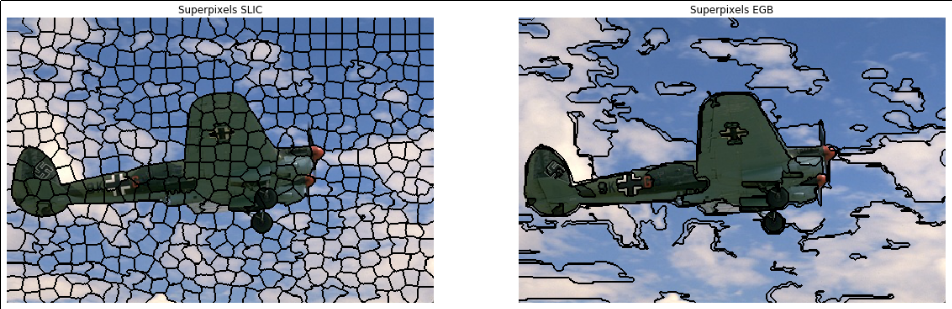
\includegraphics[width=1.\textwidth]{superpixels.png}
\caption{Imagem segmentada utilizando superpixel SLIC, com aproximadamente 500 segmentos.}
\label{fig:superpixel}
\end{figure}

A utilização de superpixels possibilita a redução de itens a serem processados, entretanto pode causar perda de informação importante. No entanto, para alguns casos, a perda de qualidade pode se justificar em relação ao ganho de velocidade obtido utilizando esse tipo de operação. Essa relação consiste então em um \textit{trade-off} entre ambas as características, sendo viáveis em alguns cenários de processamento em tempo real ou para dispositivos com baixo desempenho.

O presente trabalho tem como objetivo investigar a utilização de superpixels como passo de pré processamento para segmentação de imagens. Esse trabalho investiga se a utilização de métodos de \textit{oversegmentation} podem facilitar ou dificultar o processo de treinamento. O trabalho também tentará identificar se o treinamento utilizando imagens pré processadas obtêm resultados semelhantes àqueles utilizando imagens originais, na etapa de validação.

O presente trabalho apresenta a seguinte estrutura: a Seção \ref{sec:ref_teorico} mostra o referencial teórico para construção do trabalho, a Seção  \ref{sec:mat_metodos}, exibe os materiais e métodos utilizados nos testes; a Seção \ref{sec:testes} mostra os resultados obtidos nos testes realizados e a discussões dos mesmos; a Seção \ref{sec:conclusao} contém a conclusão do artigo, com as considerações finais.

%%%%%%%%%%%%%%%%%%%%%%%%%%%%%%%%%%%%%%%%%%%%%%%%%%%%%%%
%%%%%%%%%%%%%%%%%%%%%%%%%%%%%%%%%%%%%%%%%%%%%%%%%%%%%%%
%%%%%%%%%%%%%%%%%%%%%%%%%%%%%%%%%%%%%%%%%%%%%%%%%%%%%%%


\section{Referencial Teórico} \label{sec:ref_teorico}

%%%%%%%%%%%%%%%%%%%%%%%%%%%%%%%%%%%%%%%%%%%%%%%%%%%%%%%
%%%%%%%%%%%%%%%%%%%%%%%%%%%%%%%%%%%%%%%%%%%%%%%%%%%%%%%

\subsection{Superpixels} \label{ssec:superpixels}

Superpixels são estruturas que agrupam pixels semelhantes em conjuntos. O agrupamento possibilita a redução de complexidade das tarefas de processamento \cite{SLIC}, ao reduzir a quantidade de itens a serem processados. Os superpixels são utilizados na área de visão computacional para solução de vasto número de problemas, como detecção de contorno \cite{CONTOUR}, segmentação \cite{SEG_MERGE} e localização de objetos \cite{SEG_LOCALIZ}.

Superpixels, segundo \cite{FELZENSZWALB}, devem capturar importante grupos ou regiões, refletindo aspectos da imagem. Devem também ser executados em tempo próximo ao linear em relação a quantidade de pixels. Existem diversas abordagens para a geração de superpixels \cite{SLIC}. Dentre elas, podemos classificá-las, segundo o método de agrupamento em: 

\begin{itemize}
 \item \textit{Algoritmos baseados em grafos}: utilizam abordagem baseadas em grafos para correlação entre pixels e criação dos conjuntos. Dentre os algoritmos baseados em grafos podemos citar o \textit{Efficient Graph-Based Image Segmentation} (EGB) \cite{FELZENSZWALB};
 \item \textit{Algoritmos baseados em gradiente ascendente}: utilizam métodos de gradiente ascendente iterativamente até que os critérios de convergência correspondam a forma de um superpixel. Nesse conjunto, podemos  citar as abordagens \textit{watersheds} \cite{WATERSHEDS} \cite{SLIC}
 \item \textit{Algoritmos de clusterização iterativo}: utilizam métodos de clusterização, como o \textit{k-means}, para produção de superpixels. Um exemplo desse algoritmo é o SLIC (\textit{Simple Linear Iteravite Clustering}) \cite{SLIC}
\end{itemize}

%%%%%%%%%%%%%%%%%%%%%%%%%%%%%%%%%%%%%%%%%%%%%%%%%%%%%%%

\subsubsection{Superpixels SLIC} \label{sssec:slic}

O algoritmo SLIC utiliza um único parâmetro \textit{k}, correspondente a quantidade aproximada de superpixels. A fim de produzir tamanhos semelhantes, o intervalo analisado é $S=\sqrt{N/k}$, onde \textit{N} é o número de pixels da imagem. Os centros são movidos para o local das sementes correspondentes a posição mais baixa do gradiente em uma vizinhança de 3x3, evitando que superpixels sejam centrados nas bordas ou em um posição de ruído \cite{SLIC}. Em seguida, 
cada pixel é associado com o centro do cluster mais próximo, de modo que a região de busca se sobreponham \cite{SLIC}. A fim de aumentar o desempenho do algoritmo, a região de busca é limitada em 2 vezes o tamanho aproximado do superpixel S, gerando busca em uma área 2S x 2S \cite{SLIC}. Em seguida, um passo de atualiza os centros dos clusters e computa o erro residual E \cite{SLIC}. O algoritmo disponível na figura \ref{alg:SLIC}, resume as informações descrita nesse parágrafo.

\begin{figure}[ht]
\centering
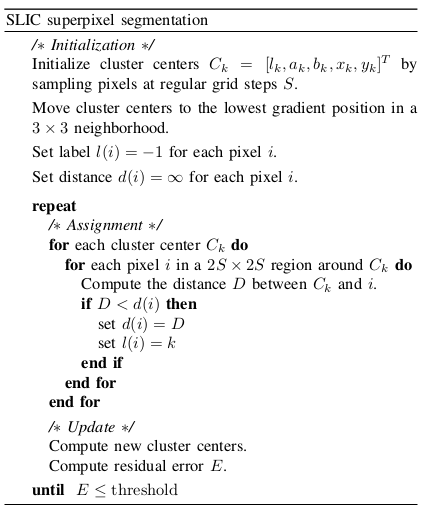
\includegraphics[width=.6\textwidth]{algoritmo_slic.png}
\caption{Algoritmo SLIC - Adaptado de \cite{SLIC}}
\label{alg:SLIC}
\end{figure}

Para o algoritmo descrito na figura \ref{alg:SLIC}, é necessário compreender o método para cálculo da medida de distância D entre os conjuntos. Devido ao algoritmo trabalhar no \textit{colorspace} CIELAB, com o espaço-plano \textit{labxy}, a posição do pixel pode assumir um intervalo de valores de acordo com o tamanho da image \ref{alg:SLIC}. Com isso, o cálculo da distância não pode ser feito utilizando uma distância euclidiana, sendo necessária uma prévia normalização da proximidade espacial e de cor. Para isso é utilizado a fórmula $D=\sqrt{d_c^2+(d_s/S)^2 \cdot m^2}$, onde $D$ corresponde a distância em 5 dimensões do espaço labxy, $d_c$ e $d_s$ correspondem à proximidade de cores e espacial; e $m^2$ corresponde a distância máxima entre cores no cluster \cite{SLIC}. Para o cálculo da distância em imagens em escala cinza, é utilizada a distância Euclidiana.

Uma etapa extra no processo de pós processamento é a união de \textit{pixels orfãos}. Esses pixels são adicionados ao cluster mais próximo usando o algoritmo de componentes conexos \cite{SLIC}.

Devido a limitação do espaço de pesquisa do algoritmo SLIC, a complexidade do algoritmo é $O(n)$, enquanto outros algoritmos que utilizam k-means para segmentação tem custo $O(k^N)$ \cite{SLIC}.

\begin{figure}[ht]
\centering
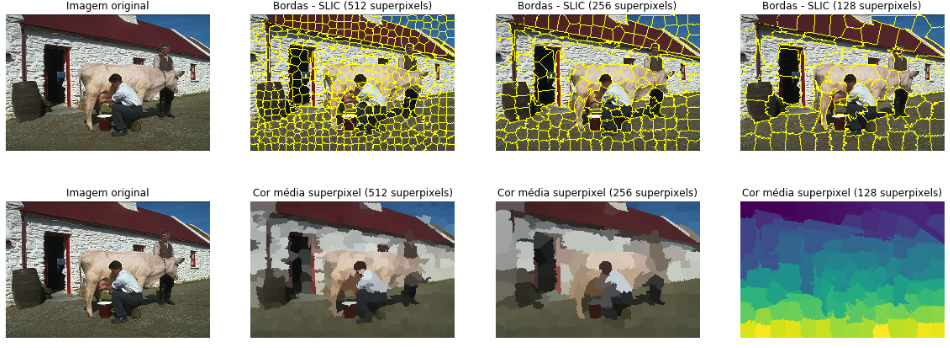
\includegraphics[width=1.\textwidth]{slic_segmentation_compare.png}
\caption{Fronteiras e coloração pelo valor médio dos superpixels SLIC/SLICO, para diferentes quantidades de superpixels}
\label{fig:SLICO}
\end{figure}

%%%%%%%%%%%%%%%%%%%%%%%%%%%%%%%%%%%%%%%%%%%%%%%%%%%%%%%

\subsubsection{Superpixels EGB} \label{sssec:slic}

Os superpixels EGB (\textit{Efficient Graph-Based Image Segmentation}) utilizam uma abordagem baseadas em grafos não direcionados. Nessa abordagem, cada pixel corresponde a um nó do grafo e a ligação entre eles ocorre por meio de arestas, com pesos não negativos, correspondente a medida de dissimilaridade \cite{FELZENSZWALB}. 

Na abordagem baseada em grafos, a segmentação $S$ é uma partição dos vértices $V$ em componentes, no qual cada região $C \in S$ corresponde a um componente conectado em um grafo $G'=(V,E')$, onde $E' \subseteq E$, ou seja, a segmentação é induzida por um conjuntos de vértices em arestas $E$ \cite{FELZENSZWALB}.

No algoritmo foi definido um predicado $D$ para avaliação da evidência de bordas entre dois componentes de uma segmentação. O algoritmo avalia a dissimilaridade entre elementos de dois componentes e os compara com elementos vizinhos em um mesmo componente, de modo que o algoritmo possa se adaptar em relação as características dos dados \cite{FELZENSZWALB}. 

Para a comparação entre as regiões é utilizada uma função de corte (\textit{threshold}) $\tau$, a fim de medir o grau de diferença entre os componentes. Esse grau deve ser superior a diferença interna mínima, evidenciando uma borda \cite{FELZENSZWALB}. A função de corte, no algoritmo, é utilizada baseado no tamanho do componente $\tau=k/|C|$, onde $|C|$ corresponde ao tamanho do componente $C$ e $k$ corresponde a um parâmetro do algoritmo \cite{FELZENSZWALB}.

O algoritmo Felzenszwalb, utilizando pesos inteiros e ordenação por contagem, pode ser executado com custo linear, com complexidade $O(nlogn)$, para qualquer método de ordenação \cite{FELZENSZWALB}.

\begin{figure}[ht]
\centering
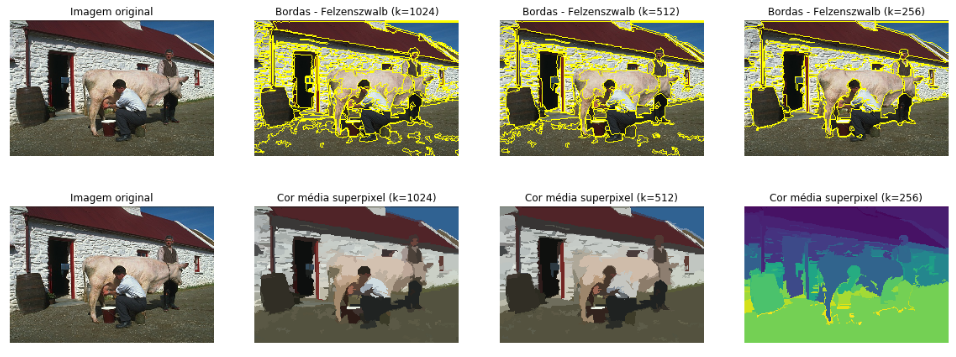
\includegraphics[width=1.\textwidth]{felz_segmentation_compare.png}
\caption{Fronteiras e coloração pelo valor médio dos superpixels Felzenszwalb, para diferentes quantidades de superpixels}
\label{fig:EGB}
\end{figure}

%%%%%%%%%%%%%%%%%%%%%%%%%%%%%%%%%%%%%%%%%%%%%%%%%%%%%%%
%%%%%%%%%%%%%%%%%%%%%%%%%%%%%%%%%%%%%%%%%%%%%%%%%%%%%%%

\subsection{Clusters} \label{sssec:clusters}

Análise de cluster é a tarega de agrupar conjunto de objetos de forma que um grupo (cluster) tenha características em comuns a outros grupos, ou clusters \cite{WIKI_CLUSTER_ANALYSIS}. Clusters hierárquicos é um método de análise de clusters a fim de buscar hierarquias entre eles. As estratégias para hierarquização de cluster se dividem em dois grupos \cite{ROKACH}:

\begin{itemize}
 \item Aglomerativo - abordagem \textit{"bottom up"}, em que a observação inicia-se no próprio cluster e os pares de clusters são unidos na medida em que se sobe na hierarquia. 
 \item Divisivo - abordagem \textit{"top down"} onde as observações iniciam-se em um cluster e são realizadas recursivamente a medida em que se desce na hierarquia.
\end{itemize}

Os algoritmos originais de cluster possuem complexidade $O(n^3)$. Alguns algoritmos, entretanto, como o SLINK, ou \textit{single-linkage}, possuem complexidade $O(n^2)$ \cite{SLINK}. O SLINK utiliza como critério de ligação (\textit{linkage}) entre os clusters a distância mínima. A fórmula $min\{d(a,b): a \in A, b \in B \}$, corresponde a distância mínima para dois pares de clusters A e B observados, onde $d$ é a métrica de distância escolhida \cite{WIKI_CLUSTER_HIERARCHY}.

A partir da aglomeração de clusters é possivel construir uma árvore hierarquica, onde os clusters são agrupados por sua similaridade. Um método de visualização dessas características é o dendrograma. 

%%%%%%%%%%%%%%%%%%%%%%%%%%%%%%%%%%%%%%%%%%%%%%%%%%%%%%%
%%%%%%%%%%%%%%%%%%%%%%%%%%%%%%%%%%%%%%%%%%%%%%%%%%%%%%%

\subsection{Segmentação de Imagens} \label{ssec:segmentacao}

Segmentação de imagens consiste em separar uma imagem em regiões, idealmente correspondente a objetos reais \cite{ZHANG2008}. Esse passo é utilizado como passo de processamento de imagens, vídeos e aplicações de visão computacional. Também consiste em um importante passo na tentativa de explicar uma imagem por meio de algoritmos \cite{ZHANG2008}.

Extensiva pesquisa é realizada e muitas abordagens e algoritmos são utilizados, com bons resultados para um conjunto ou classes de imagens \cite{ZHANG2008}. A fim de facilitar a pesquisa, alguns trabalhos foram desenvolvidos para criação de um conjunto de imagens com suas respectivas segmentações manuais. A base BSDS500 (\textit{Berkeley Segmentation Data Set and Benchmarks 500}) provê uma base de imagens para pesquisa em segmentação e detecção de bordas. \cite{BSDS500}. Essa base de dados é uma extensão da base BSDS300, com 200 novas imagens para avaliação \cite{BSDS500}.

A fim de avaliar a efetividade das segmentações, tradicionalmente são utilizados métodos subjetivos, como a visualização humana, responsável por comparar a qualidade da segmentação ou métodos supervisionados, onde uma segmentação é comparada em relação a uma imagem manualmente segmentada \cite{ZHANG2008}. Projetos de detecção automática, como o SEISM (\textit{Supervised Evaluation of Image Segmentation Methods}) permitem a avaliação da segmentação, usando a recuperação de precisão para bordas e a recuperação de precisão para objetos e peças \cite{SEISM}

%%%%%%%%%%%%%%%%%%%%%%%%%%%%%%%%%%%%%%%%%%%%%%%%%%%%%%%
%%%%%%%%%%%%%%%%%%%%%%%%%%%%%%%%%%%%%%%%%%%%%%%%%%%%%%%
%%%%%%%%%%%%%%%%%%%%%%%%%%%%%%%%%%%%%%%%%%%%%%%%%%%%%%%

\section{Materiais e Métodos} \label{sec:mat_metodos}

Para realização dos testes foram escolhidos os algoritmos de \textit{oversegmentation} SLIC e Felzenszwalb. Os algoritmos possuem características diferentes: o SLIC é capaz de produzir superpixels em formas regulares, porém não é tão preciso ao separar os conjuntos por similaridade; por outro lado, o Felzenszwalb, produz pixels irregulares, porém é mais aderente às diferenças de cores entre pixels.

A utilização de ambos os algoritmos busca obter um melhor desempenho em relação a utilização  dos algoritmos de forma isolada. O primeiro algoritmo aplicado às imagens foi o algoritmo SLIC, gerando superpixels de formas regulares. Em seguida, foi realizada recoloração da imagem utilizando o valor do pixel médio do superpixel. Em seguida, foi aplicado às imagens o método de Felzenszwalb.

Os resultados dos algoritmo utilizando a composição entre os métodos SLIC e Felzenszwalb foram comparados aos melhores resultados obtidos para os algoritmos executados separadamente. O método descrito foi aplicado à base de dados BSDB500 e comparados com as imagens manualmente segmentadas (\textit{ground-truth}).

%Após a execução dos algoritmos, foram gerados \textit{clusters} com as correlações entre os grupos, utilizando o algoritmo SLINK (\textit{single-linkage}). Os cortes foram realizados em diversos níveis da hierarquia e os resultados foram avaliados manualmente, a fim de encontrar bons parâmetros para o algoritmo. 

Os algoritmos SLIC e Felzenszwalb utilizados para confecção desse trabalho foram obtidos pela biblioteca Scikit-Image \footnote{http://scikit-image.org/docs/dev/api/skimage.segmentation.html}. O algoritmo de geração de cluster SLINK foi obtido na biblioteca Scipy.org \footnote{https://docs.scipy.org/doc/scipy-0.18.1/reference/generated/scipy.cluster.hierarchy.linkage.html}. Os códigos fontes gerados estão disponíveis publicamente no Github \footnote{https://github.com/falreis/image-segm}.

%%%%%%%%%%%%%%%%%%%%%%%%%%%%%%%%%%%%%%%%%%%%%%%%%%%%%%%

\subsection{Avaliação de Resultados} \label{sec:aval_resultados}

Para avaliação das imagens, foi primeiramente utilizada a classificação visual, comparando a qualidade dos resultados. Em seguida utilizou-se um método de comparação de precisão e revocação, com auxílio de um algoritmo para avaliação do resultado. \footnote{Código disponível em: https://github.com/Htiango/Image-Segmentation/blob/master/main/eval\_boundary.py}

O método de precisão é um método de classificação binária, onde a precisão (textit{prediction}) corresponde à ``fração de instâncias recuperadas que são relevantes'', enquanto revocação (\textit{recall}), corresponde ``a fração de instâncias relevantes que são recuperadas'' \cite{WIKI_PREC_RECALL}. Ambos os métodos são avaliados juntos para que possam identificar 4 tipos de valores possíveis:

\begin{itemize}
 \item Verdadeiros Positivos - correspondem aos valores que foram corretamente classificados como positivos;
 \item Falsos Negativos - correspondem aos valores que foram classificados incorretamente como negativos;
 \item Falsos Positivos - correspondem aos valores que foram classificados incorretamente como positivos;
 \item Verdadeiros Negativos - correspondem aos valores que foram classificados corretamente como negativos \cite{WIKI_PREC_RECALL};
\end{itemize}

A classificação descrita acima está ilustrada na figura \ref{fig:PREC_RECALL}. 

\begin{figure}[ht]
\centering
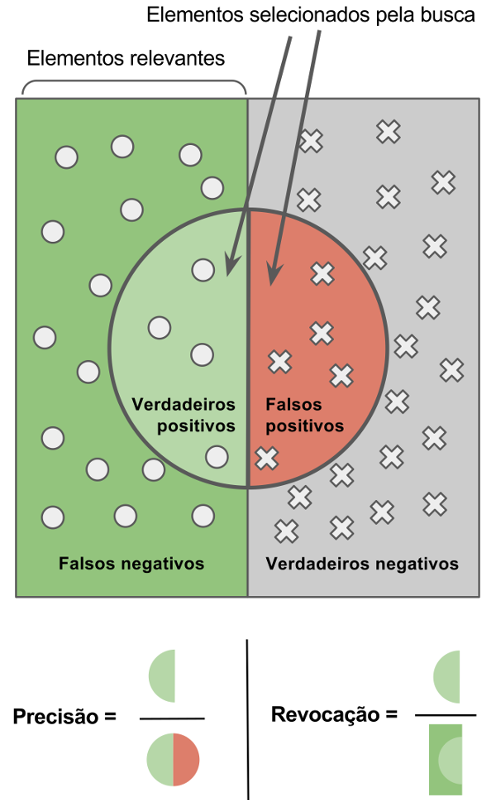
\includegraphics[width=0.4\textwidth]{precision_recall.png}
\caption{Precisão e revocação. Adaptado de \cite{WIKI_PREC_RECALL}}
\label{fig:PREC_RECALL}
\end{figure}

A classificação de precisão e revocação pode ser dada por uma média harmônica, chamada de \textit{F-measure} ou \textit{F-score} balanceada. Essa medida é dada pela fórmula \cite{WIKI_PREC_RECALL}:

\begin{equation}
 F=2 \cdot \frac{precis \cdot revoc}{precis+revoc}
\end{equation}

A medida é aproximadamente a média quando seus valores estão próximos, porém o valor é baixo quando as médias estão distantes, favorecendo métodos com baixo número de falsos positivos e verdadeiros negativos \cite{WIKI_PREC_RECALL}

%%%%%%%%%%%%%%%%%%%%%%%%%%%%%%%%%%%%%%%%%%%%%%%%%%%%%%%
%%%%%%%%%%%%%%%%%%%%%%%%%%%%%%%%%%%%%%%%%%%%%%%%%%%%%%%
%%%%%%%%%%%%%%%%%%%%%%%%%%%%%%%%%%%%%%%%%%%%%%%%%%%%%%%


\section{Testes, Resultados e Discussões} \label{sec:testes}

%%%%%%%%%%%%%%%%%%%%%%%%%%%%%%%%%%%%%%%%%%%%%%%%%%%%%%%
%%%%%%%%%%%%%%%%%%%%%%%%%%%%%%%%%%%%%%%%%%%%%%%%%%%%%%%

\begin{figure}[ht]
\centering
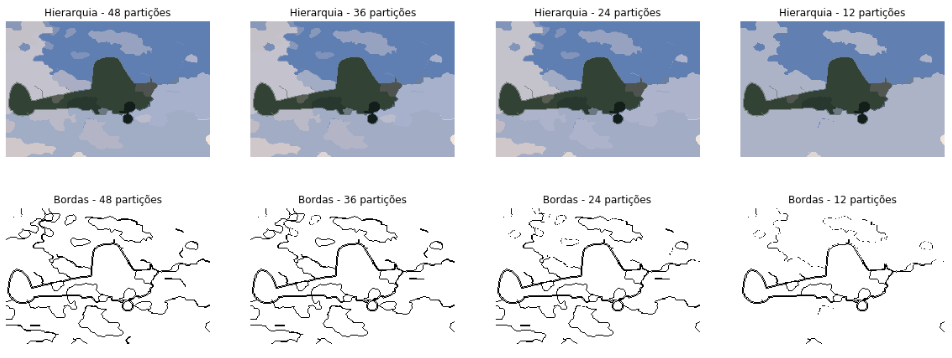
\includegraphics[width=1.\textwidth]{slic_hierarquia_particoes.png}
\caption{Fronteiras das Hierarquia de partições utilizando superpixel SLICO.}
\label{alg:SLIC}
\end{figure}

%%%%%%%%%%%%%%%%%%%%%%%%%%%%%%%%%%%%%%%%%%%%%%%%%%%%%%%
%%%%%%%%%%%%%%%%%%%%%%%%%%%%%%%%%%%%%%%%%%%%%%%%%%%%%%%
%%%%%%%%%%%%%%%%%%%%%%%%%%%%%%%%%%%%%%%%%%%%%%%%%%%%%%%

\section{Conclusão} \label{sec:conclusao}

%%%%%%%%%%%%%%%%%%%%%%%%%%%%%%%%%%%%%%%%%%%%%%%%%%%%%%%
%%%%%%%%%%%%%%%%%%%%%%%%%%%%%%%%%%%%%%%%%%%%%%%%%%%%%%%
%%%%%%%%%%%%%%%%%%%%%%%%%%%%%%%%%%%%%%%%%%%%%%%%%%%%%%%

\bibliographystyle{sbc}
\bibliography{sbc-template}

\end{document}
